\documentclass[11pt]{article}
\usepackage[margin=1in]{geometry}
\usepackage{fontspec,booktabs,array,graphicx,adjustbox,amsmath}
\usepackage[font=small,labelfont=bf]{caption}
\usepackage{natbib,xurl}
\usepackage[hidelinks]{hyperref}
\usepackage{setspace}
\setstretch{1.15}
\renewcommand{\floatpagefraction}{0.8}
\graphicspath{{../figs/}}
\newcommand{\DeletionRange}{[-20.17, -19.88]}
\newcommand{\DemN}{505}
\newcommand{\FavorBaseline}{28.5}
\newcommand{\FavorCI}{[-23.5, -13.6]}
\newcommand{\FavorEstimate}{-18.6}
\newcommand{\FavorN}{911}
\newcommand{\FavorTreated}{9.9}
\newcommand{\FullN}{1,625}
\newcommand{\HighwayDemBounds}{[64.7, 65.1]}
\newcommand{\HighwayDemCI}{[61.5, 68.3]}
\newcommand{\HighwayDemCount}{499}
\newcommand{\HighwayDemEstimate}{65.0}
\newcommand{\HighwayDemLarger}{35.0}
\newcommand{\HighwayDemN}{768}
\newcommand{\HighwayMissing}{6}
\newcommand{\HighwayN}{1,380}
\newcommand{\HighwayObserved}{1,374}
\newcommand{\HighwayPoolBounds}{[68.2, 68.6]}
\newcommand{\HighwayPoolCI}{[66.0, 70.9]}
\newcommand{\HighwayPoolCount}{941}
\newcommand{\HighwayPoolEstimate}{68.5}
\newcommand{\HighwayPoolLarger}{31.5}
\newcommand{\HighwayPoolN}{1,374}
\newcommand{\HighwayRepBounds}{[72.6, 73.1]}
\newcommand{\HighwayRepCI}{[69.3, 76.3]}
\newcommand{\HighwayRepCount}{442}
\newcommand{\HighwayRepEstimate}{72.9}
\newcommand{\HighwayRepLarger}{27.1}
\newcommand{\HighwayRepN}{606}
\newcommand{\IncomeDemBaseline}{49.5}
\newcommand{\IncomeDemCI}{[-29.1, -19.1]}
\newcommand{\IncomeDemEstimate}{-24.1}
\newcommand{\IncomeDemN}{505}
\newcommand{\IncomeDemTreated}{25.4}
\newcommand{\IncomeMatchedBaseline}{47.7}
\newcommand{\IncomeMatchedCI}{[-24.9, -16.3]}
\newcommand{\IncomeMatchedEstimate}{-20.6}
\newcommand{\IncomeMatchedN}{743}
\newcommand{\IncomeMatchedTreated}{27.0}
\newcommand{\IncomeN}{911}
\newcommand{\IncomePoolBaseline}{46.7}
\newcommand{\IncomePoolCI}{[-23.9, -16.1]}
\newcommand{\IncomePoolEstimate}{-20.0}
\newcommand{\IncomePoolN}{911}
\newcommand{\IncomePoolTreated}{26.7}
\newcommand{\IncomeRepBaseline}{43.2}
\newcommand{\IncomeRepCI}{[-21.2, -8.6]}
\newcommand{\IncomeRepEstimate}{-14.9}
\newcommand{\IncomeRepN}{406}
\newcommand{\IncomeRepTreated}{28.3}
\newcommand{\IncomeStrictBaseline}{49.4}
\newcommand{\IncomeStrictCI}{[-27.0, -18.0]}
\newcommand{\IncomeStrictEstimate}{-22.5}
\newcommand{\IncomeStrictN}{713}
\newcommand{\IncomeStrictTreated}{26.9}
\newcommand{\IncomeUnobserved}{0}
\newcommand{\IncomeWeightedBaseline}{48.7}
\newcommand{\IncomeWeightedCI}{[-25.8, -15.7]}
\newcommand{\IncomeWeightedEstimate}{-20.8}
\newcommand{\IncomeWeightedN}{743}
\newcommand{\IncomeWeightedTreated}{28.0}
\newcommand{\JobsAllBaseline}{50.9}
\newcommand{\JobsAllCI}{[5.6, 10.8]}
\newcommand{\JobsAllEstimate}{8.2}
\newcommand{\JobsAllN}{1,624}
\newcommand{\JobsAllTreated}{59.1}
\newcommand{\JobsBlackBaseline}{39.3}
\newcommand{\JobsBlackCI}{[18.0, 34.1]}
\newcommand{\JobsBlackEstimate}{26.1}
\newcommand{\JobsBlackN}{168}
\newcommand{\JobsBlackTreated}{65.3}
\newcommand{\JobsMissing}{1}
\newcommand{\JobsWhiteBaseline}{52.3}
\newcommand{\JobsWhiteCI}{[3.2, 9.3]}
\newcommand{\JobsWhiteEstimate}{6.3}
\newcommand{\JobsWhiteN}{1,159}
\newcommand{\JobsWhiteTreated}{58.6}
\newcommand{\MatchedN}{1,000}
\newcommand{\MatchedPostN}{859}
\newcommand{\NonpartisanBaseline}{37.2}
\newcommand{\NonpartisanCI}{[-12.9, 4.7]}
\newcommand{\NonpartisanEstimate}{-4.1}
\newcommand{\NonpartisanN}{141}
\newcommand{\NonpartisanTreated}{33.2}
\newcommand{\OpposeBaseline}{34.0}
\newcommand{\OpposeCI}{[23.7, 36.1]}
\newcommand{\OpposeEstimate}{29.9}
\newcommand{\OpposeN}{911}
\newcommand{\OpposeTreated}{63.9}
\newcommand{\PartyDifferenceCI}{[-17.2, -1.2]}
\newcommand{\PartyDifferenceEstimate}{-9.2}
\newcommand{\PartyDifferenceN}{911}
\newcommand{\PermutationP}{0.0001}
\newcommand{\PostN}{1,052}
\newcommand{\PostRate}{64.7}
\newcommand{\PrePostChangeN}{70}
\newcommand{\RepN}{406}

\hypersetup{pdfauthor={Gaurav Sood and Alexander G. Theodoridis},
  pdftitle={Pareto Partisan? Relative Gains and Support for Public Policy}}
\title{Pareto Partisan?\\Relative Gains and Support for Public Policy}
\author{Gaurav Sood \and Alexander G. Theodoridis}
\date{}
\begin{document}
\maketitle
\begin{abstract}
\noindent If people prefer more for both sides to less for both, everyone should choose a plan that gives both sides more. Two exercises in the 2018 Cooperative Congressional Election Study examine departures from that benchmark. In a highway choice, only \HighwayDemLarger{}\% of Democrats and \HighwayRepLarger{}\% of Republicans selected the plan allocating more to both groups of states. The rest preferred less for both sides but a relative advantage for their own. This is a large departure from the allocation benchmark, although preferring lower public spending could also explain it. A post-election experiment holds the own-party income gain at 5\% while raising the opposing party's gain from 3\% to 7\%. Support should not fall if respondents value their own side's gain and are indifferent to, or welcome, additional gains for opponents. Instead, support changes by \IncomePoolEstimate{} points on a 0--100 scale (95\% CI \IncomePoolCI{}), with declines in both parties. These results challenge the sufficiency of favorable absolute gains for policy support. They are consistent with concern for relative partisan advantage, but do not identify spite separately from aversion to falling behind or establish a Pareto ranking of net welfare.
\end{abstract}

\section{Absolute gains and partisan advantage}
A natural benchmark for policy choice is that people prefer more for both sides to less for both. Under that benchmark, a plan that gives both groups larger benefits should be chosen by everyone, not merely by a majority. Our question is how far observed choices depart from that prediction when the plan delivering more also leaves the respondent's party behind.

The benchmark has explicit conditions. Let $x$ denote the stated benefit to one's own side and $y$ the benefit to the other side. If respondents evaluate only these benefits, prefer a larger $x$, and do not dislike a larger $y$, then $x_A>x_B$ and $y_A>y_B$ imply a preference for $A$. This includes a purely own-group-oriented respondent who is indifferent to opponents' gains. With understood amounts, no choice error, and no other relevant differences, everyone should select $A$. The prediction is 100\% selection of the plan delivering more, not 50\%. A choice share far below that benchmark calls for an explanation even if the larger plan were to win a majority.
% The 100% and 50% values specify theoretical benchmarks, not empirical estimates.

The pre-election highway question supplies this comparison in stated allocations. One plan gives more to both groups of states but leaves the respondent's side behind; the other gives less to both but leaves it ahead. Only \HighwayDemLarger{}\% of Democrats and \HighwayRepLarger{}\% of Republicans select the larger plan. These departures from universal selection are descriptively large. They are not, by themselves, estimates of how many people reject a Pareto improvement in welfare: public spending has costs, and the larger plan may not make every person better off after financing and opportunity costs.

The post-election income experiment tests a related implication. It holds the own-party gain at 5\% and assigns the opposing party a gain of either 3\% or 7\%. If respondents care only about their own party's stated gain, their support should be unchanged; if they also welcome additional gains for opponents, it should not decrease. Unlike the highway item, respondents evaluate one assigned plan rather than choose between both. The benchmark is therefore a nonnegative effect on support, not universal selection of the higher-opposition-gain plan. The observed effect is negative in both parties.

These comparisons separate absolute gains from relative advantage, but do not uniquely identify a motive. Favoring one's own side is not the same as wanting the other side to suffer; experiments separating opportunities to help allies from opportunities to harm opponents illustrate that distinction \citep{amira2021}. Social-preference models likewise distinguish concern for absolute payoffs, inequality, relative disadvantage, and others' welfare \citep{fehr1999,charness2002}. Here the absolute gap between the stated gains is the same on either side of each comparison, while the identity of the group ahead changes. Symmetric dislike of unequal gains alone would not favor own-party advantage. Dislike of falling behind could. Incomes before the policy are not specified, so equal gaps in percentage gains need not imply equal gaps in income levels.

A strict welfare interpretation requires more than these exercises supply. Highway allocations go to groups of states, not directly to each partisan individual. The income scenarios describe average gains for voters from each party, not guaranteed net gains for every person. We therefore distinguish a benchmark of monotonic preferences over the displayed group benefits from a verified Pareto improvement in individual welfare. The experiments also involve hypothetical evaluations, not decisions with respondents' own money at stake.

\section{Data, assignment, and measurement}
The data come from the University of California, Merced module of the 2018 Cooperative Congressional Election Study (CCES). YouGov administered the survey online. The CCES pre-election wave ran from September 27 through November 5, and its post-election wave from November 7 through December 3 \citep{cces2018}. The full team delivery contains \FullN{} respondents; a matched delivery contains \MatchedN{} of the same respondents. Shared analysis fields agree after matching by the vendor's unique identifier. The public replication file contains one record per respondent, a matched-sample indicator, and the original numeric response codes for the retained fields.
% Field dates above are from the official CCES 2018 guide and agree with the original timestamps.

CCES matching selects respondents from online opt-in samples to resemble a population frame; it is not direct probability sampling of respondents from that frame. The main analysis uses the full delivery without weights to describe the observed choices and estimate the experimental comparison. We also report the matched sample unweighted and with its supplied team weights. Those alternatives change the analyzed population or its composition. No separate post-election team weight is present in these deliveries, so the team-weighted post-election results are a sensitivity analysis, not an attrition-adjusted national estimate. The CCES guide recommends wave-appropriate weights for population descriptions \citep{cces2018}.

The highway question was asked of \HighwayN{} partisans, including leaners; \HighwayObserved{} answered and \HighwayMissing{} skipped. Nonpartisans were not asked. The income experiment was administered to \PostN{} post-election participants, of whom \IncomeN{} identified with or leaned toward a party in that wave: \DemN{} Democrats and \RepN{} Republicans. Every assigned participant has an observed income-plan response. The remaining pre-election respondents have neither a recorded income assignment nor an outcome; we do not count their absence as a response to the income treatment. The experiment describes those who reached the post-election module, not all original respondents.

Party identification is measured separately in the two waves. We use the pre-election seven-point measure for highway eligibility and the post-election identification and leaning questions for the income comparison. The updated measure exactly matches the delivered partisan routing: Democrats see Democratic voters gaining 5\%, and Republicans see Republican voters gaining 5\%. Using pre-election identification would misclassify some respondents' relationship to the displayed beneficiaries. Nonpartisans have no defined own-party gain and are analyzed separately in the appendix.

The module questionnaire instructs random assignment to income images. The delivered arms are nearly evenly split within each partisan group (Table~\ref{tab:assignment}). The materials do not provide execution logs or a complete final routing script. Our causal interpretation requires the 3\%-versus-7\% assignment to have been randomized within partisan routing, as the instruction and delivered assignments imply. It also assumes that respondents received their assigned image and did not affect one another's responses. We do not infer a causal effect of party membership from comparisons between Democrats and Republicans. The analyses are exploratory; no preregistered analysis plan accompanies the materials.

\begin{table}[!htbp]
\centering\small
\caption{Income experiment: assignment and response counts among partisans.}
\label{tab:assignment}
\begin{tabular}{lrrr}
\toprule
Respondents & Opposition gain & Assigned & Observed \\
\midrule
Democrats & 3\% & 256 & 256 \\
Democrats & 7\% & 249 & 249 \\
Republicans & 3\% & 203 & 203 \\
Republicans & 7\% & 203 & 203 \\
\bottomrule
\end{tabular}

\begin{minipage}{\linewidth}\footnotesize
Own-party income gain is 5\% in every arm. Party includes leaners and uses the post-election identification questions. Assignment counts refer to the full delivery, before restricting to the matched sample.
\end{minipage}
\end{table}

\section{How far choices depart from the allocation benchmark}
The highway item presents two named proposals and asks which the respondent supports. The Smith plan allocates \$11 billion to states associated with the respondent's own party and \$12 billion to the opposing party's states. The Williams plan allocates \$10 billion and \$9 billion, respectively. Democrats receive an image naming blue states first; Republicans receive the corresponding image naming red states first. The images describe states, not payments directly to partisan individuals. The questionnaire calls for randomizing the order of the response options; no response-order variable is available in the delivery.

Choosing Williams gives up \$1 billion for one's own side's states and \$3 billion for the other side's states. Total stated funding falls from \$23 billion to \$19 billion, while the own-side allocation moves from \$1 billion behind to \$1 billion ahead. These arithmetic differences are properties of the displayed proposals, not estimates from the data.
% Dollar amounts and differences above follow directly from data/materials/highway/{Blue,Red}.png.

Against a benchmark in which everyone selects Smith, only \HighwayPoolLarger{}\% do so. The remaining \HighwayPoolEstimate{}\% select Williams, a \HighwayPoolEstimate{}-percentage-point shortfall from universal selection of the larger allocation. This shortfall is a description of choices, not a separately identified rate of partisan spite. In party-specific counts, Williams is chosen by \HighwayDemCount{} of \HighwayDemN{} Democrats and \HighwayRepCount{} of \HighwayRepN{} Republicans (Table~\ref{tab:highway}). The corresponding shares are \HighwayDemEstimate{}\% (95\% Wilson interval \HighwayDemCI{}) and \HighwayRepEstimate{}\% (\HighwayRepCI{}). Including all skipped answers at either extreme gives a pooled choice-share range of \HighwayPoolBounds{}\%; the small amount of item nonresponse does not account for the majority preference. This range describes possible completions of the observed sample, not sampling uncertainty.

\begin{table}[!htbp]
\centering\small
\caption{Highway choice: selecting the larger Smith plan.}
\label{tab:highway}
\begin{tabular}{lrr}
\toprule
Respondents & Larger plan / answered & Percent [95\% CI] \\
\midrule
Democrats & 269/768 & 35.0 [31.7, 38.5] \\
Republicans & 164/606 & 27.1 [23.7, 30.7] \\
Pooled & 433/1374 & 31.5 [29.1, 34.0] \\
\bottomrule
\end{tabular}

\begin{minipage}{\linewidth}\footnotesize
Unweighted shares among respondents answering the item, including leaners. Smith gives more to both sides but leaves the respondent's side behind. The monotonic-allocation benchmark predicts 100\% selection of Smith. Intervals are binomial Wilson intervals and do not account for nonprobability sample selection.
\end{minipage}
\end{table}

The choice is consistent with valuing relative partisan advantage enough to accept a smaller gross allocation for one's own side. But it is not a randomized estimate of the effect of partisan labels: everyone sees a partisan allocation, and the two plans differ in both distribution and total spending. A preference for lower government spending, judgments about which states need funding, or reactions to the named proposals could also affect the choice. Both plans have the same absolute dollar gap between the two groups of states; a symmetric preference for equal allocations does not by itself favor Williams. The data establish a preference for the displayed smaller plan, not the motive behind that preference. We do not test the exact 100\% benchmark with a binomial $p$-value: under an error-free universal-choice model, even one contrary answer is impossible. The informative quantities are the size of the departure, its persistence across sample definitions, and the competing explanations. Without comprehension measures or a neutral version of the same choice, we cannot separate choice error from preferences that depart from the benchmark.

\section{When opponents gain more and one's own gain stays fixed}
The post-election images describe a new economic plan under which the average voter from the respondent's party receives a 5\% income increase. The average voter from the opposing party receives either 3\% or 7\%. The images use the same headline, photograph, and source label and name the own-party beneficiary first. Respondents rate the plan from strongly support to strongly oppose. These are researcher-provided scenarios, not verified news reports. Additional image variants in the materials describe an isolated 5\% gain or equal gains; none has a corresponding assigned arm in the delivered data.

We reverse and rescale the five-category response to 0--100, with 100 meaning strongly support, 50 neither support nor oppose, and 0 strongly oppose. A difference of 25 points is one response category. The primary estimate is the mean support difference between the 7\% and 3\% opposition-gain conditions, averaged across parties using their fixed shares among all eligible income-experiment partisans. Each party's contrast compares independently assigned respondents, not the same person's response to both plans. We use independent cell-mean variances and Welch--Satterthwaite 95\% intervals. The appendix supplies the formulas and checks the interpretation using response categories rather than only the rescaled mean.

Raising opponents' gain changes support by \IncomePoolEstimate{} points (95\% CI \IncomePoolCI{}). Estimated support falls from \IncomePoolBaseline{} to \IncomePoolTreated{} (Table~\ref{tab:income}), despite the unchanged own-party gain. The changes are \IncomeDemEstimate{} points among Democrats (\IncomeDemCI{}) and \IncomeRepEstimate{} among Republicans (\IncomeRepCI{}). These are substantial changes within the observed scale. The comparison does not require respondents to prefer lower gains for their own side: that gain is the same in both conditions.

\begin{table}[!htbp]
\centering\small
\caption{Income experiment: policy support when opponents gain more.}
\label{tab:income}
\adjustbox{max width=\linewidth}{\begin{tabular}{lrrrr}
\toprule
Respondents & Opposition 3\% & Opposition 7\% & Difference [95\% CI] & $n$ \\
\midrule
Democrats & 49.5 & 25.4 & -24.1 [-29.1, -19.1] & 505 \\
Republicans & 43.2 & 28.3 & -14.9 [-21.2, -8.6] & 406 \\
Pooled & 46.7 & 26.7 & -20.0 [-23.9, -16.1] & 911 \\
\bottomrule
\end{tabular}
}
\begin{minipage}{\linewidth}\footnotesize
Own-party gain is 5\%. Support runs from 0 (strongly oppose) to 100 (strongly support). Entries are arm means and 7\%-minus-3\% differences with 95\% Welch intervals. Pooled means and differences standardize to the full experimental partisan composition; $n$ counts both arms.
\end{minipage}
\end{table}

The result is visible in the response categories. The standardized share somewhat or strongly supporting the plan falls from \FavorBaseline{}\% to \FavorTreated{}\%, a \FavorEstimate{}-percentage-point difference (\FavorCI{}). The share somewhat or strongly opposing rises from \OpposeBaseline{}\% to \OpposeTreated{}\%. Thus the result is not solely a consequence of treating the categories as equally spaced. The full distributions appear in Appendix Figure~\ref{fig:distribution}.

\begin{figure}[!htbp]
\centering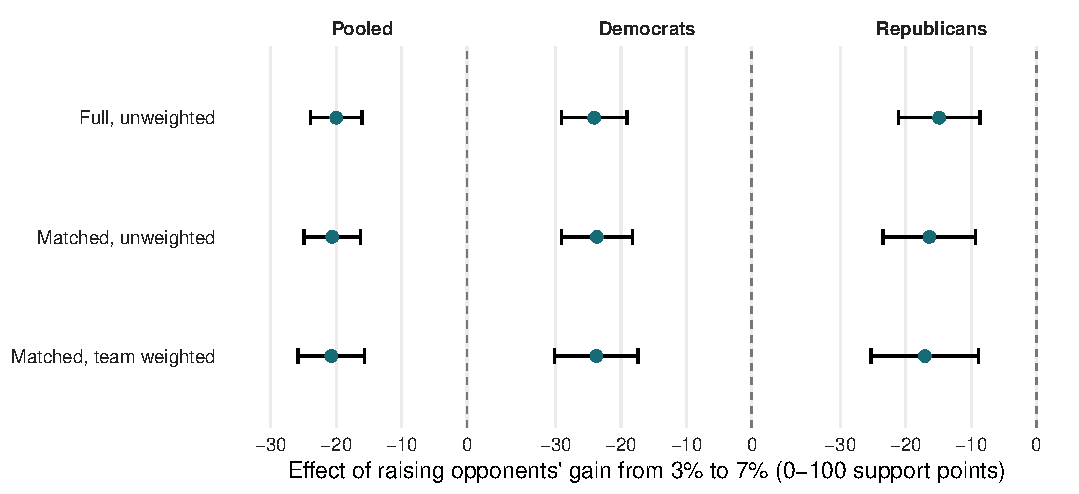
\includegraphics[width=\linewidth]{income_effects.pdf}
\caption{Income experiment: larger opposition gains reduce support under each sample and weighting choice. Points are 7\%-minus-3\% differences, keeping the own-party gain at 5\%; bars are 95\% intervals. All panels include leaners. Unweighted estimates use Welch intervals; team-weighted estimates use fixed-weight HC3 cell variances. Each pooled estimate uses its own eligible sample's party shares.}
\label{fig:effects}
\end{figure}

The pooled estimate is \IncomeMatchedEstimate{} (\IncomeMatchedCI{}) in the matched sample and \IncomeWeightedEstimate{} (\IncomeWeightedCI{}) with team weights. Restricting the full sample to respondents who directly identify as Democrats or Republicans, excluding leaners, gives \IncomeStrictEstimate{} (\IncomeStrictCI{}). These comparisons preserve the direction and substantial magnitude of the response while changing the represented sample. Exact single-respondent deletions, holding the full sample's party shares fixed, give estimates from \DeletionRange{}. A within-party permutation check gives $p=\PermutationP{}$; this check assumes exchangeability under the stated assignment mechanism. It does not verify implementation of the randomizer.

The estimated reduction is larger among Democrats. The Democrat-minus-Republican effect difference is \PartyDifferenceEstimate{} points (\PartyDifferenceCI{}). This exploratory comparison describes heterogeneity across the observed groups and stories; it does not establish that one party is generally more spiteful. Both groups' estimates answer the same concrete question and show lower support when opponents move ahead.

\section{What the choices establish}
The two exercises fall short of distinct benchmark predictions. Universal selection of the larger highway allocation would follow from valuing own-side gains without disliking gains for the other side, provided other costs and attributes were held fixed. The observed larger-plan choice share is only \HighwayPoolLarger{}\%. In the income experiment, a fixed own-party gain would imply unchanged support under purely own-group preferences, and additional opposing-party gains would not reduce support under monotonic preferences over both groups' stated benefits. Instead, support falls substantially. A plan becomes less attractive when the opposition's stated gain increases enough to put it ahead. The highway result makes the possible consequence more concrete: many respondents select a plan that funds both sets of states less but gives their own side the larger allocation. Together, the results challenge an account of policy support based only on the absolute material gains described for one's own side.

They do not uniquely identify spite. In the income experiment, larger opposition gains and the loss of relative advantage occur together. Dislike of falling behind, a desire to restrain opponents, judgments of deservingness, or skepticism about the plan could generate the observed response. With no politically neutral beneficiary condition, we cannot determine how much of that response is distinctive to partisan rivalry rather than a more general concern about relative position. In the highway question, the lower total budget adds a separate fiscal interpretation. The income experiment removes that particular budget comparison, but does not provide a full account of perceived policy costs or credibility.

The distinction between group allocations and personal sacrifice also matters. The highway question concerns funding for groups of states; the income question concerns average voters from each party. Neither puts respondents' money at risk or asks them to choose between two personally paid amounts. We therefore cannot infer willingness to lose a specified amount of personal income, calculate the welfare cost of partisan animus, or treat a stated plan preference as an actual policy decision.

A stronger test of costly partisan spite would separate the beneficiary's party from the respondent's absolute gain, vary opponents' gains without always reversing relative rank, and specify financing or other costs. A neutral-group comparison would distinguish partisan rivalry from general disadvantage aversion. The present evidence supports a narrower but consequential conclusion: relative partisan gains enter expressed policy evaluations, and providing one's own side with a positive gain is not enough to secure support when the other side gains more.

\section*{Data and replication}
The public replication repository is \url{https://github.com/soodoku/pareto_partisan}. It contains numeric analysis extracts, original stimulus images and questionnaires, the R analysis, generated results, and this manuscript. Original survey deliveries are retained separately. Running \texttt{make check} rebuilds the outputs and runs linting and tests. Every estimated number in the prose is generated from the analysis tables.

\bibliographystyle{apalike}
\bibliography{references}
\clearpage
\appendix
\section{Sensitivity and response distributions}
\begin{table}[!htbp]
\centering\small
\caption{Highway choice: percent selecting the smaller plan.}
\adjustbox{max width=\linewidth}{\begin{tabular}{lrrr}
\toprule
Sample / identity & Democrats & Republicans & Pooled \\
\midrule
Full + leaners & 65.0 [61.5, 68.3] & 72.9 [69.3, 76.3] & 68.5 [66.0, 70.9] \\
Full strict & 66.7 [62.9, 70.3] & 73.8 [69.6, 77.7] & 69.7 [66.8, 72.3] \\
Matched + leaners & 64.7 [60.3, 68.8] & 73.3 [68.5, 77.6] & 68.4 [65.2, 71.4] \\
Matched strict & 65.7 [60.9, 70.3] & 74.6 [69.1, 79.4] & 69.4 [65.8, 72.8] \\
Matched weighted + leaners & 65.5 [60.5, 70.5] & 74.1 [68.8, 79.5] & 69.5 [65.8, 73.1] \\
Matched weighted strict & 65.7 [60.0, 71.3] & 74.6 [68.2, 80.9] & 69.5 [65.4, 73.7] \\
\bottomrule
\end{tabular}
}
\begin{minipage}{\linewidth}\footnotesize
Intervals are 95\% Wilson intervals for unweighted shares and fixed-weight HC3 $t$ intervals for weighted shares, truncated to the response scale. ``Strict'' uses direct party identification; ``+ leaners'' includes independent leaners. Weighted shares use the supplied team weights on the matched sample. These choices change the sample or its composition.
\end{minipage}
\end{table}

\begin{table}[!htbp]
\centering\small
\caption{Income experiment: 7\%-minus-3\% differences in support.}
\adjustbox{max width=\linewidth}{\begin{tabular}{lrrr}
\toprule
Sample / identity & Democrats & Republicans & Pooled \\
\midrule
Full + leaners & -24.1 [-29.1, -19.1] & -14.9 [-21.2, -8.6] & -20.0 [-23.9, -16.1] \\
Full strict & -24.0 [-29.6, -18.4] & -20.4 [-27.8, -13.0] & -22.5 [-27.0, -18.0] \\
Matched + leaners & -23.7 [-29.1, -18.3] & -16.4 [-23.5, -9.3] & -20.6 [-24.9, -16.3] \\
Matched strict & -24.2 [-30.2, -18.2] & -20.1 [-28.3, -11.8] & -22.5 [-27.4, -17.6] \\
Matched weighted + leaners & -23.8 [-30.1, -17.4] & -17.1 [-25.3, -8.8] & -20.8 [-25.8, -15.7] \\
Matched weighted strict & -22.4 [-29.3, -15.5] & -21.1 [-30.6, -11.7] & -21.8 [-27.5, -16.2] \\
\bottomrule
\end{tabular}
}
\begin{minipage}{\linewidth}\footnotesize
All outcomes run from 0 to 100. Intervals are 95\% Welch intervals for unweighted estimates and fixed-weight HC3 $t$ intervals for weighted estimates. Each pooled estimate standardizes to its eligible partisan composition. The team weights are not a separate adjustment for post-election attrition.
\end{minipage}
\end{table}

\begin{figure}[!htbp]
\centering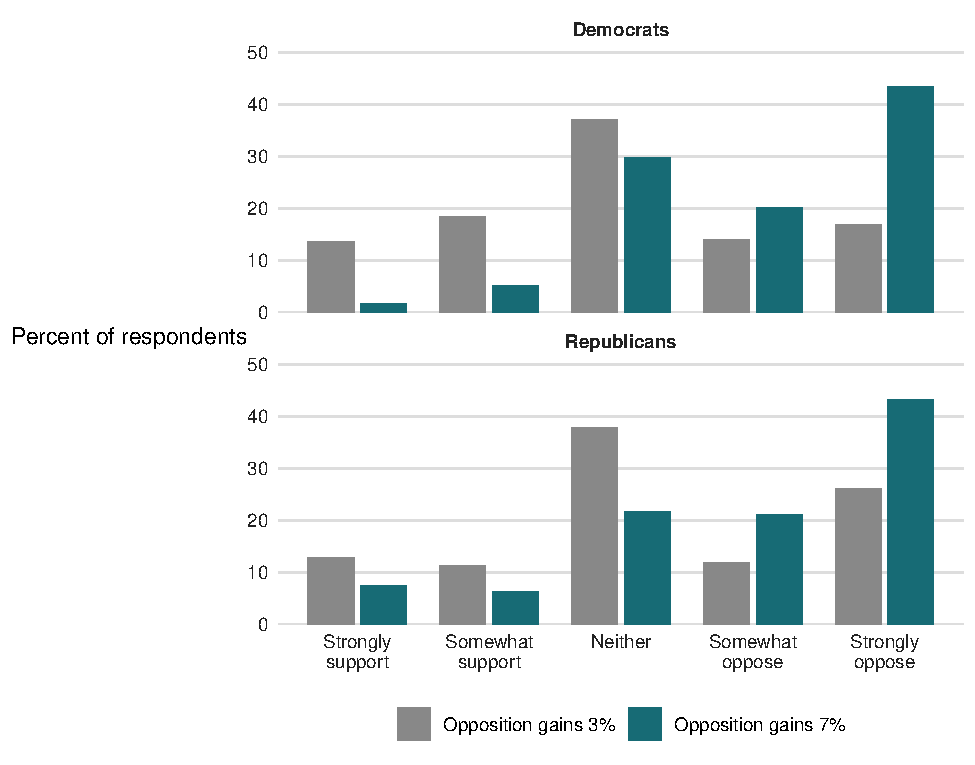
\includegraphics[width=.88\linewidth]{income_distribution.pdf}
\caption{Income-plan responses by party and opposing-party gain. Bars show unweighted percentages among all assigned partisans in each arm; own-party gain is always 5\%. Every assigned respondent answered. The scale displays the full response distribution rather than uncertainty for each category.}
\label{fig:distribution}
\end{figure}

\clearpage
\section{Nonpartisans and the separate race-and-jobs vignette}
The \NonpartisanN{} post-election respondents without a partisan side also received income images. Averaging within the party named as receiving 5\%, the effect of increasing the other party's gain is \NonpartisanEstimate{} support points (\NonpartisanCI{}). There is no own-versus-opposition interpretation for these respondents. The interval includes both a meaningful decline and a modest increase; this imprecise estimate does not demonstrate indifference to relative gains.

A separate pre-election item describes a congressional primary candidate's jobs plan. The plan raises the income of an average Black family making \$50,000 by 7\% and an average White family making \$50,000 by 5\%, or reverses those percentages. The questionnaire calls for randomizing the Black-versus-White version. The recorded candidate-party field follows respondents' pre-election party, including leaners; it is not independently randomized among partisans. The question asks how likely respondents are to vote for the candidate, using six categories from extremely likely to extremely unlikely. We code these from 100 to 0, respectively. \JobsMissing{} skipped response is excluded; the difference is between the Black-advantage and White-advantage versions.
% Jobs stimulus amounts and percentages come from data/materials/UCM_Module.docx.

The pooled estimate is \JobsAllEstimate{} points (\JobsAllCI{}; Table~\ref{tab:jobs}). Among White respondents it is \JobsWhiteEstimate{} (\JobsWhiteCI{}); among Black respondents it is \JobsBlackEstimate{} (\JobsBlackCI{}). These are exploratory subgroup comparisons, with unadjusted intervals. Unlike the partisan income experiment, this item changes both groups' gains. For Black and White respondents, their racial group's described gain changes as well, so the item does not isolate a response to the other group's gain with one's own held fixed. It is not a second estimate of the partisan contrast or a direct measure of costly sacrifice. The questionnaire also contains a typographical inconsistency in the White-advantage text; the deployed survey script is not available to resolve it.

\begin{table}[!htbp]
\centering\small
\caption{Jobs vignette: stated likelihood of voting for the candidate.}
\label{tab:jobs}
\adjustbox{max width=\linewidth}{\begin{tabular}{lrrrr}
\toprule
Respondents & White advantage & Black advantage & Difference [95\% CI] & $n$ \\
\midrule
All & 50.9 & 59.1 & 8.2 [5.6, 10.8] & 1624 \\
White & 52.3 & 58.6 & 6.3 [3.2, 9.3] & 1159 \\
Black & 39.3 & 65.3 & 26.1 [18.0, 34.1] & 168 \\
Other races & 51.8 & 57.4 & 5.6 [-0.5, 11.7] & 297 \\
Democrat & 49.0 & 65.1 & 16.1 [12.6, 19.6] & 771 \\
Republican & 58.4 & 56.6 & -1.8 [-6.0, 2.5] & 608 \\
\bottomrule
\end{tabular}
}
\begin{minipage}{\linewidth}\footnotesize
Full-sample unweighted means and Black-advantage-minus-White-advantage differences on a 0--100 scale, with 95\% Welch intervals. Party includes leaners. Race and party subgroups overlap; differences in statistical significance are not tests of differences between groups. This is a separate randomized vignette with a different outcome and payoff structure.
\end{minipage}
\end{table}

\section{Estimation and validation}
For the income experiment, let $p$ index respondent party and $a\in\{0,1\}$ indicate the 3\% and 7\% opposing-party gain conditions. With $s_p$ equal to the party's share in the full eligible analysis sample, the estimate is
\[
\widehat\tau=\sum_p s_p(\overline Y_{p1}-\overline Y_{p0}).
\]
Its unweighted variance is $\sum_{p,a}s_p^2s_{pa}^2/n_{pa}$, where $s_{pa}^2$ and $n_{pa}$ are the outcome variance and count in each cell. Writing the summands as $v_{pa}$, the Welch degrees of freedom are $(\sum v_{pa})^2/\sum[v_{pa}^2/(n_{pa}-1)]$. Each respondent contributes one outcome to a contrast. The between-party effect difference uses all four independent cells with coefficients $(-1,1,1,-1)$ in Democrat-low, Democrat-high, Republican-low, Republican-high order.

Weighted estimates use the supplied team weights in cell means and in the eligible party shares. Within a cell, with normalized weights $h_i=w_i/\sum_iw_i$, the HC3 variance is $\sum_i\{h_i(Y_i-\overline Y_w)/(1-h_i)\}^2$. The weighted reference degrees of freedom are the number of observed respondents minus the number of compared cells. These calculations treat weights and eligible party shares as fixed. They omit uncertainty from sample selection, weight estimation, and the choice of these particular stimuli.

The pooled support-scale income contrast is the principal experimental summary. Binary support, binary opposition, party differences, strict-identifier restrictions, and jobs-vignette subgroups are secondary or exploratory; their intervals are not adjusted for searching across those comparisons. The results do not depend on selecting a single subgroup or response threshold. The permutation check uses 9,999 within-party reassignments with seed 20261004 and includes the observed assignment in its tail probability. Its resolution is $1/10{,}000$.
% Permutation draws and seed are fixed analysis settings in R/analysis.R.

The tests verify code directions, structural nonresponse, original and matched sample counts, and exact partisan routing. Party-specific differences reproduce independent Welch tests; pooled unweighted and weighted estimates reproduce saturated regressions with HC2 and HC3 covariance estimators, respectively. Simulated data check interval coverage for a known effect. The generated tables retain arm distributions, sample alternatives, party transitions, pre-treatment balance summaries, and fixed-share case-deletion ranges. Balance summaries diagnose the recorded assignment; they do not prove that the randomizer operated as intended or determine which covariates enter the estimate.
\end{document}
